% Ana Mo Alvarez Catala
\begin{table}[h]
    \centering
    \begin{tabular}{lr}
        \textbf{Cuenta de Resultados - 4ª Decisión} & \textbf{€} \\
        \hline
        \textbf{Ingresos por ventas}                & \textbf{529530} \\
        Valor Stock inicial                         & 1201907 \\
        Componentes comprados                       & 18990 \\
        Adquisición de materias primas              & 1452750 \\
        Funcionamiento máquinas                     & 47059 \\
        Salarios mecanizado                         & 76050 \\
        Salarios montaje                            & 57798 \\
        Control de calidad                          & 1264 \\
        Transporte                                  & 19700 \\
        Menos valor de stock final                  & 2297752 \\
        \cline{2-2}
        \textbf{Coste de las ventas}                & 577766 \\
        \cline{2-2}
        \textbf{Beneficio Bruto}                    & -48236 \\
        Gastos generales                            & 439961 \\
        Seguros recibidos                           & 0 \\
        Amortización                                & 39438 \\
        \cline{2-2}
        \textbf{EBIT}                               & -527635 \\
        Ingresos financieros                        & 0 \\
        \textbf{Gastos financieros}                 & \textbf{30824} \\
        \cline{2-2}
        \textbf{Beneficio antes de impuestos}       & \textbf{-558459} \\
        Impuestos                                   & 0 \\
        \cline{2-2}
        \textbf{Resultado neto}                     & \textbf{-558459} \\
        \textbf{Beneficio por acción (cents)}       & \textbf{-13,961475} \\
        \textbf{Pago de dividendos}                 & \textbf{0} \\
        \cline{2-2}
        Transferido a reservas                      & -558459 \\
        Reservas acumuladas                         & -1546290 \\
        \cline{2-2}
        \textbf{Reservas totales}                   & \textbf{-2104749}
    \end{tabular}
\end{table}

\begin{table}[h]
    \centering
    \begin{tabular}{|c|r|}
        \hline
        Margen Explotación  & -99,64 \% \\
        Margen Operativo    & -105,46 \% \\
        Margen Neto         & -105,46 \% \\
        ROA                 & -11,32 \% \\
        ROE                 & -29,47 \% \\
        Rotación            & 11,36 \% \\
        Endeudamiento       & 145,94 \% \\
        \hline
    \end{tabular}
\end{table}

\section*{El Espejismo del Crecimiento y la Asfixia por Insolvencia Técnica}
Tras un inicio de año marcado por escasez de materias primas y una caída de ventas, este segundo trimestre se intentó proyectar hacia una corrección e intento de levantamiento. A través de la decisión para el segundo trimestre de 2018 se consiguió un incremento bastante alto en la facturación pasando de 139.975€ a 529.530€. Este incremento del 289\% a pesar de ser una buena noticia, es un dato engañoso, siendo un espejismo de crecimiento. Este crecimiento tan grande realmente llevo consigo la entrada en una fase de insolvencia técnica, ya que se deterioró el patrimonio y la liquidez, demostrando que aumentar la cuota de mercado sin una estructura de costes solo sirve para multiplicar las pérdidas.

\section*{De la Parálisis por Escasez al Colapso por Sobreabastecimiento}
Para la decisión del segundo trimestre se pudo observar que existía una falta de stock, las cuales paralizaron las ventas. Esta falta de stock fue derivada de la inexistencia de materias primas. Ante esta situación la dirección de operación realizó una decisión agresiva, abasteciendo con 21.000 unidades de materias primas para el segundo trimestres y 1.000 unidades para el siguiente trimestre.

El valor del inventario de materiales se disparó casi duplicándose, pasando de 1.183.207€ a 2.275.022€, siendo un sobrestock ineficiente. Esta decisión fue en contra de InudsMoney, debido a que se inmovilizó casi el 50\% del activo total en estanterías, bajando la liquidez de la caja y convirtiendo el activo corriente en activos improductivos que generaban costes de almacenamiento y riesgo de obsolescencia. Desde el punto de vista del ratio ROA (Retorno sobre Activos), que seguía negativo con un valor de -11\%, por lo que la decisión fue desacertada. No se puede cambiar la liquidez de caja de IndusMoney en un activo no corriente que no rota.

\section*{El Error de Financiar Inmovilizado con Línea de Crédito}
En un intento de aumento de la plantilla contratando a 5 nuevos trabajadores tomada por el departamento de recursos humanos, el departamento de finanzas empezó a pensar en una expansión más a futuro a partir de la decisión de contratación. Se amplió por tanto la fábrica en 275 metros cuadrados. El error vino de la mano de la ampliación del inmovilizado sin contar con una financiación adecuada. Lo que conllevó un descubierto de 1.401.318€, es decir, se activó un crédito de emergencia.
Fue un error la financiación de activos fijos con deuda a cortísimo plazo, ya que el descubierto del banco tiene un interés alto. Esta situación aumentó el ratio de endeudamiento duplicándolo, pasando de un preocupante 43\% a un alarmante ratio de endeudamiento de 146\%. IndusMoney ya no se financia con recursos propios y ahora la empresa pertenece a sus acreedores bancarios, sobreviviendo con unos gastos financieros que ascienden a 30.824€ duplicando los gastos del anterior cuatrimestre.


\begin{figure}[h]
  \centering
  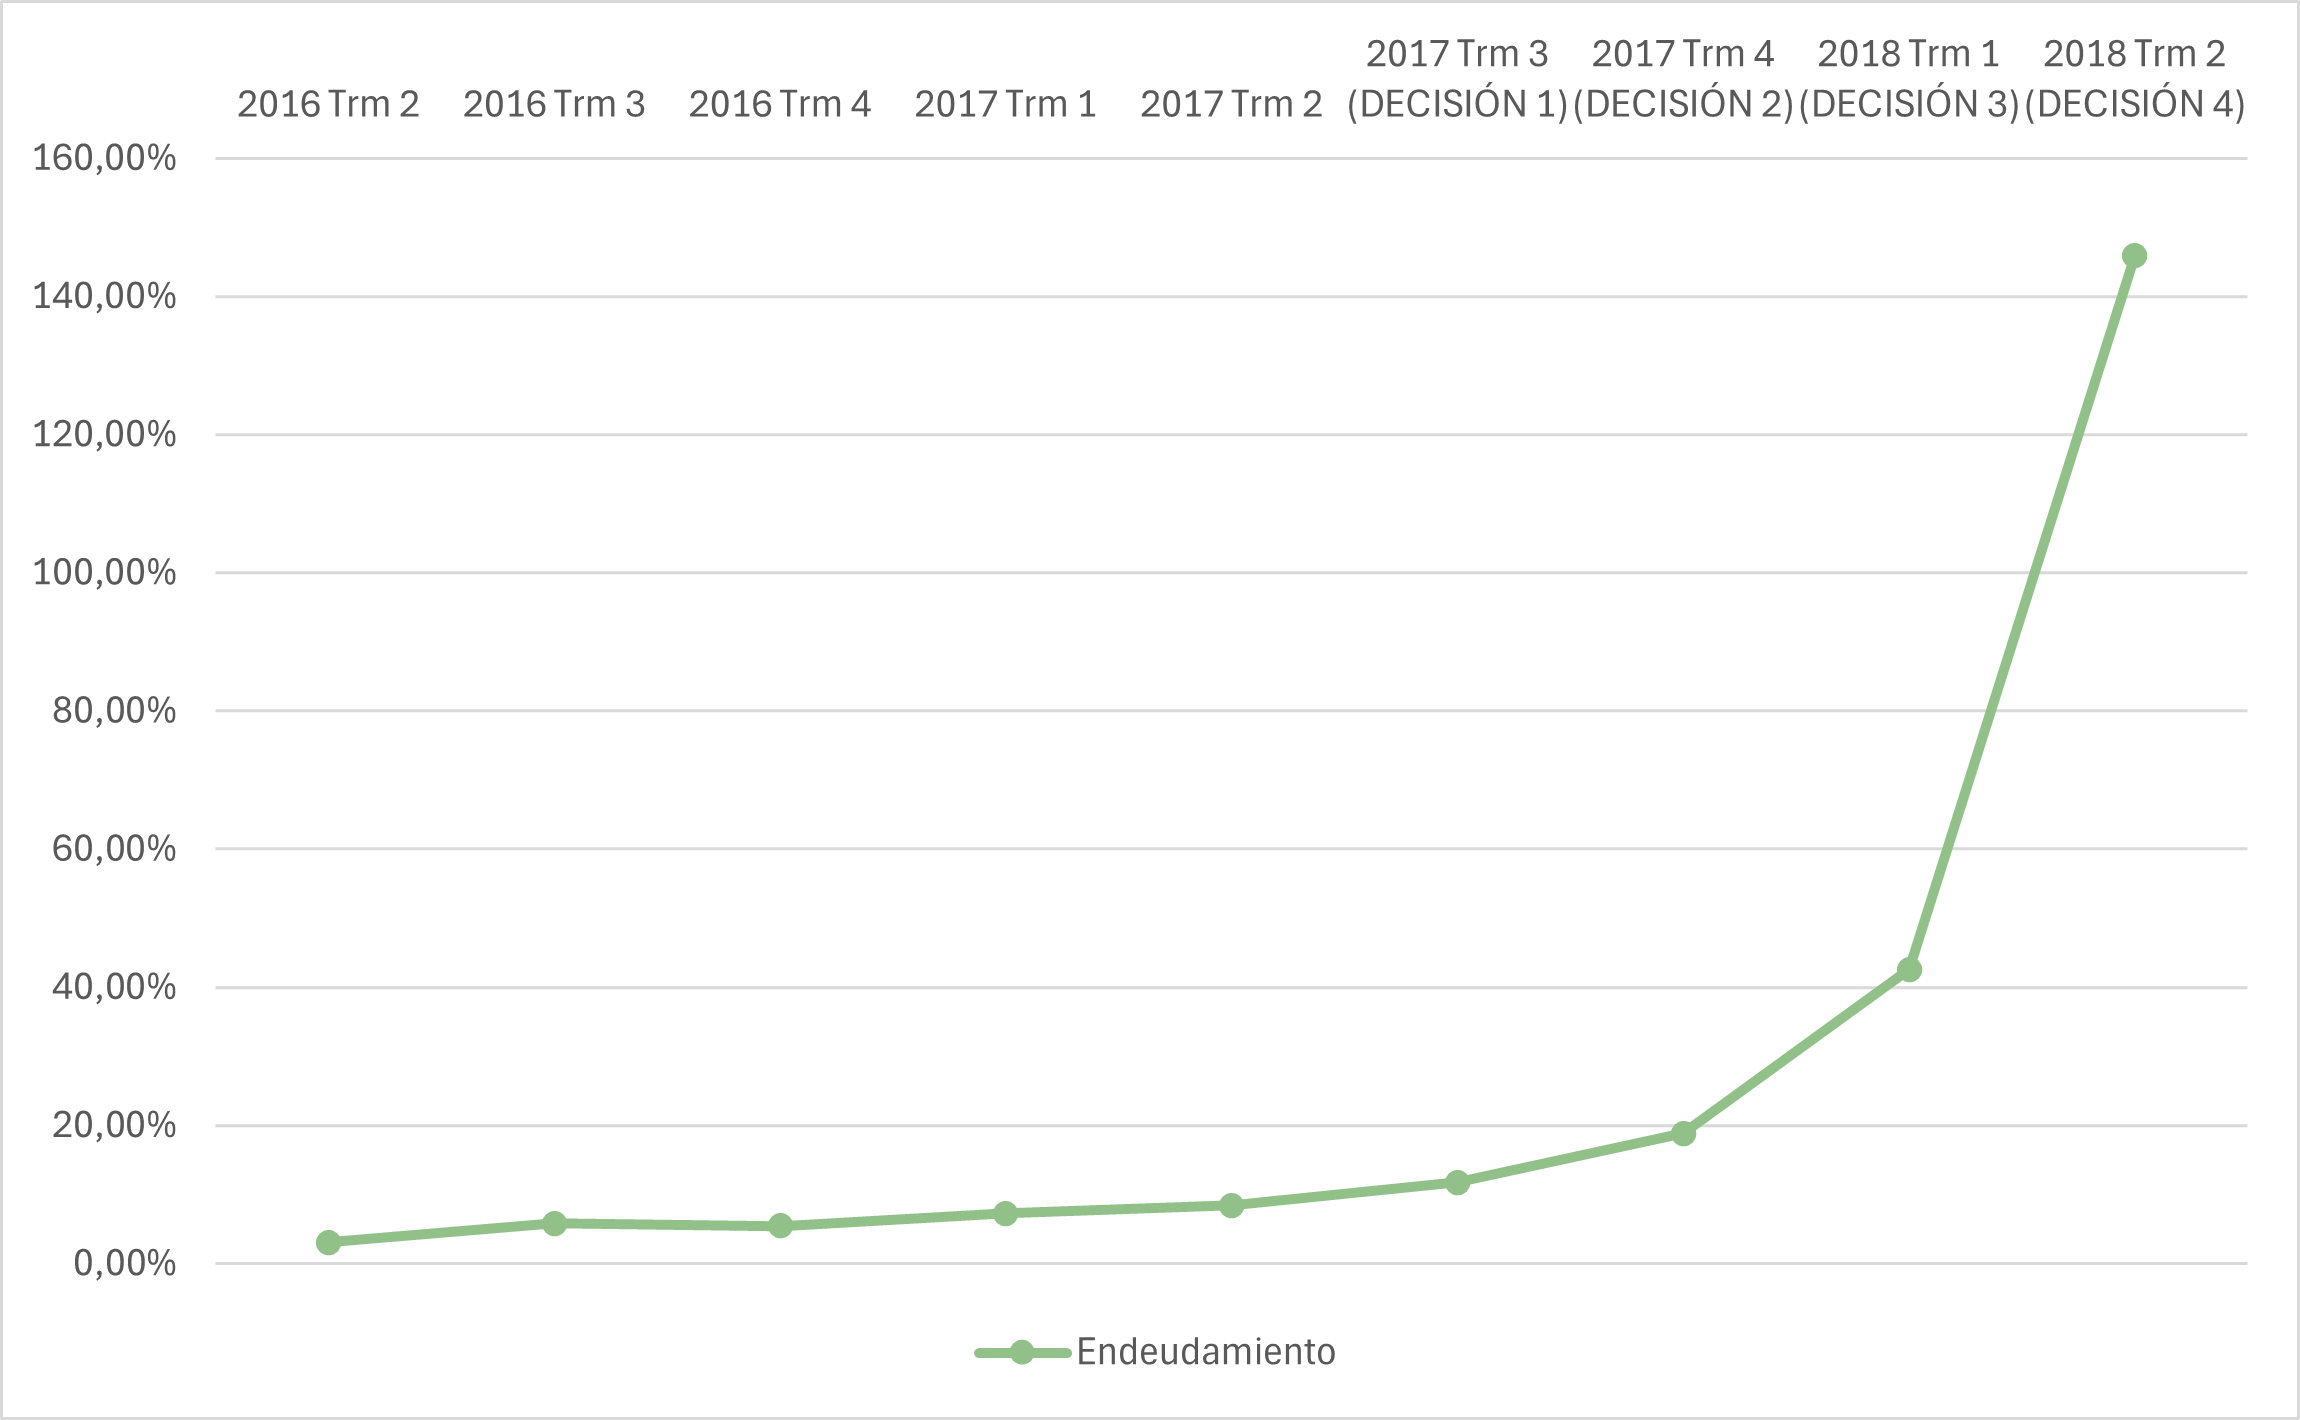
\includegraphics[width= \columnwidth]{Imagenes/decision4_endeudamiento.png}
\end{figure}

\section*{Los Costes Devoran a los Ingresos}
A pesar de la reactivación de ventas con el esfuerzo de marketing y el aumento de precios de algunos productos en los diferentes mercados, la estructura de costes sigue estando mal planteada. El beneficio bruto de -48.236€ sigue estando en negativo, aunque mucho menor que en el anterior semestre. Este dato revela que el coste directo de producción supera a los ingresos generados. 

El coste de los productos era mayor al esperado debido a la decisión de mantener un turno de trabajo y recurrir a la subcontratación de los productos. La decisión de recursos humanos y de operaciones no fue de la mano, creyendo que la falta de stock en el primer cuatrimestre del año fue el fallo primordial. Esta dualidad de pagar a los trabajadores de la empresa IndusMoney y además a la subcontratación disparó el coste de ventas hasta un valor de 577.766€.

Analizando el EBIT con un valor negativo de -527.635€ y la amortización de 39.438€, da un valor de EBITDA muy negativo de 488.197€. Estas cifras hacen ver que la situación de IndusMoney está en números rojos sin tener en cuenta ni los intereses, ni los impuestos, ni la amortización. Confirmando que si el “corazón” del negocio no funciona (que los costes del producto no sobrepasen a los ingresos) la operativa diaria de la empresa está destruyendo caja, independientemente de la financiación utilizada.

\section*{Deterioro del Patrimonio y el Fondo de Maniobra}
El resultado neto negativo ha llevado a tener las reservas totales de la empresa con un valor de -2.104.749€. Sumado a los indicadores de rentabilidad el ROE de -29\% y el ROA de -11\%, demuestran que hay un apalancamiento financiero. Al ser el coste de la deuda superior a la rentabilidad de los activos, se empieza a perder más rápido el patrimonio neto. Originando una reducción del Patrimonio Neto hasta un valor de 1.895.251€, lo que significa que se han gastado más del 50\% del capital social original de los accionistas.

\begin{figure}[h]
  \centering
  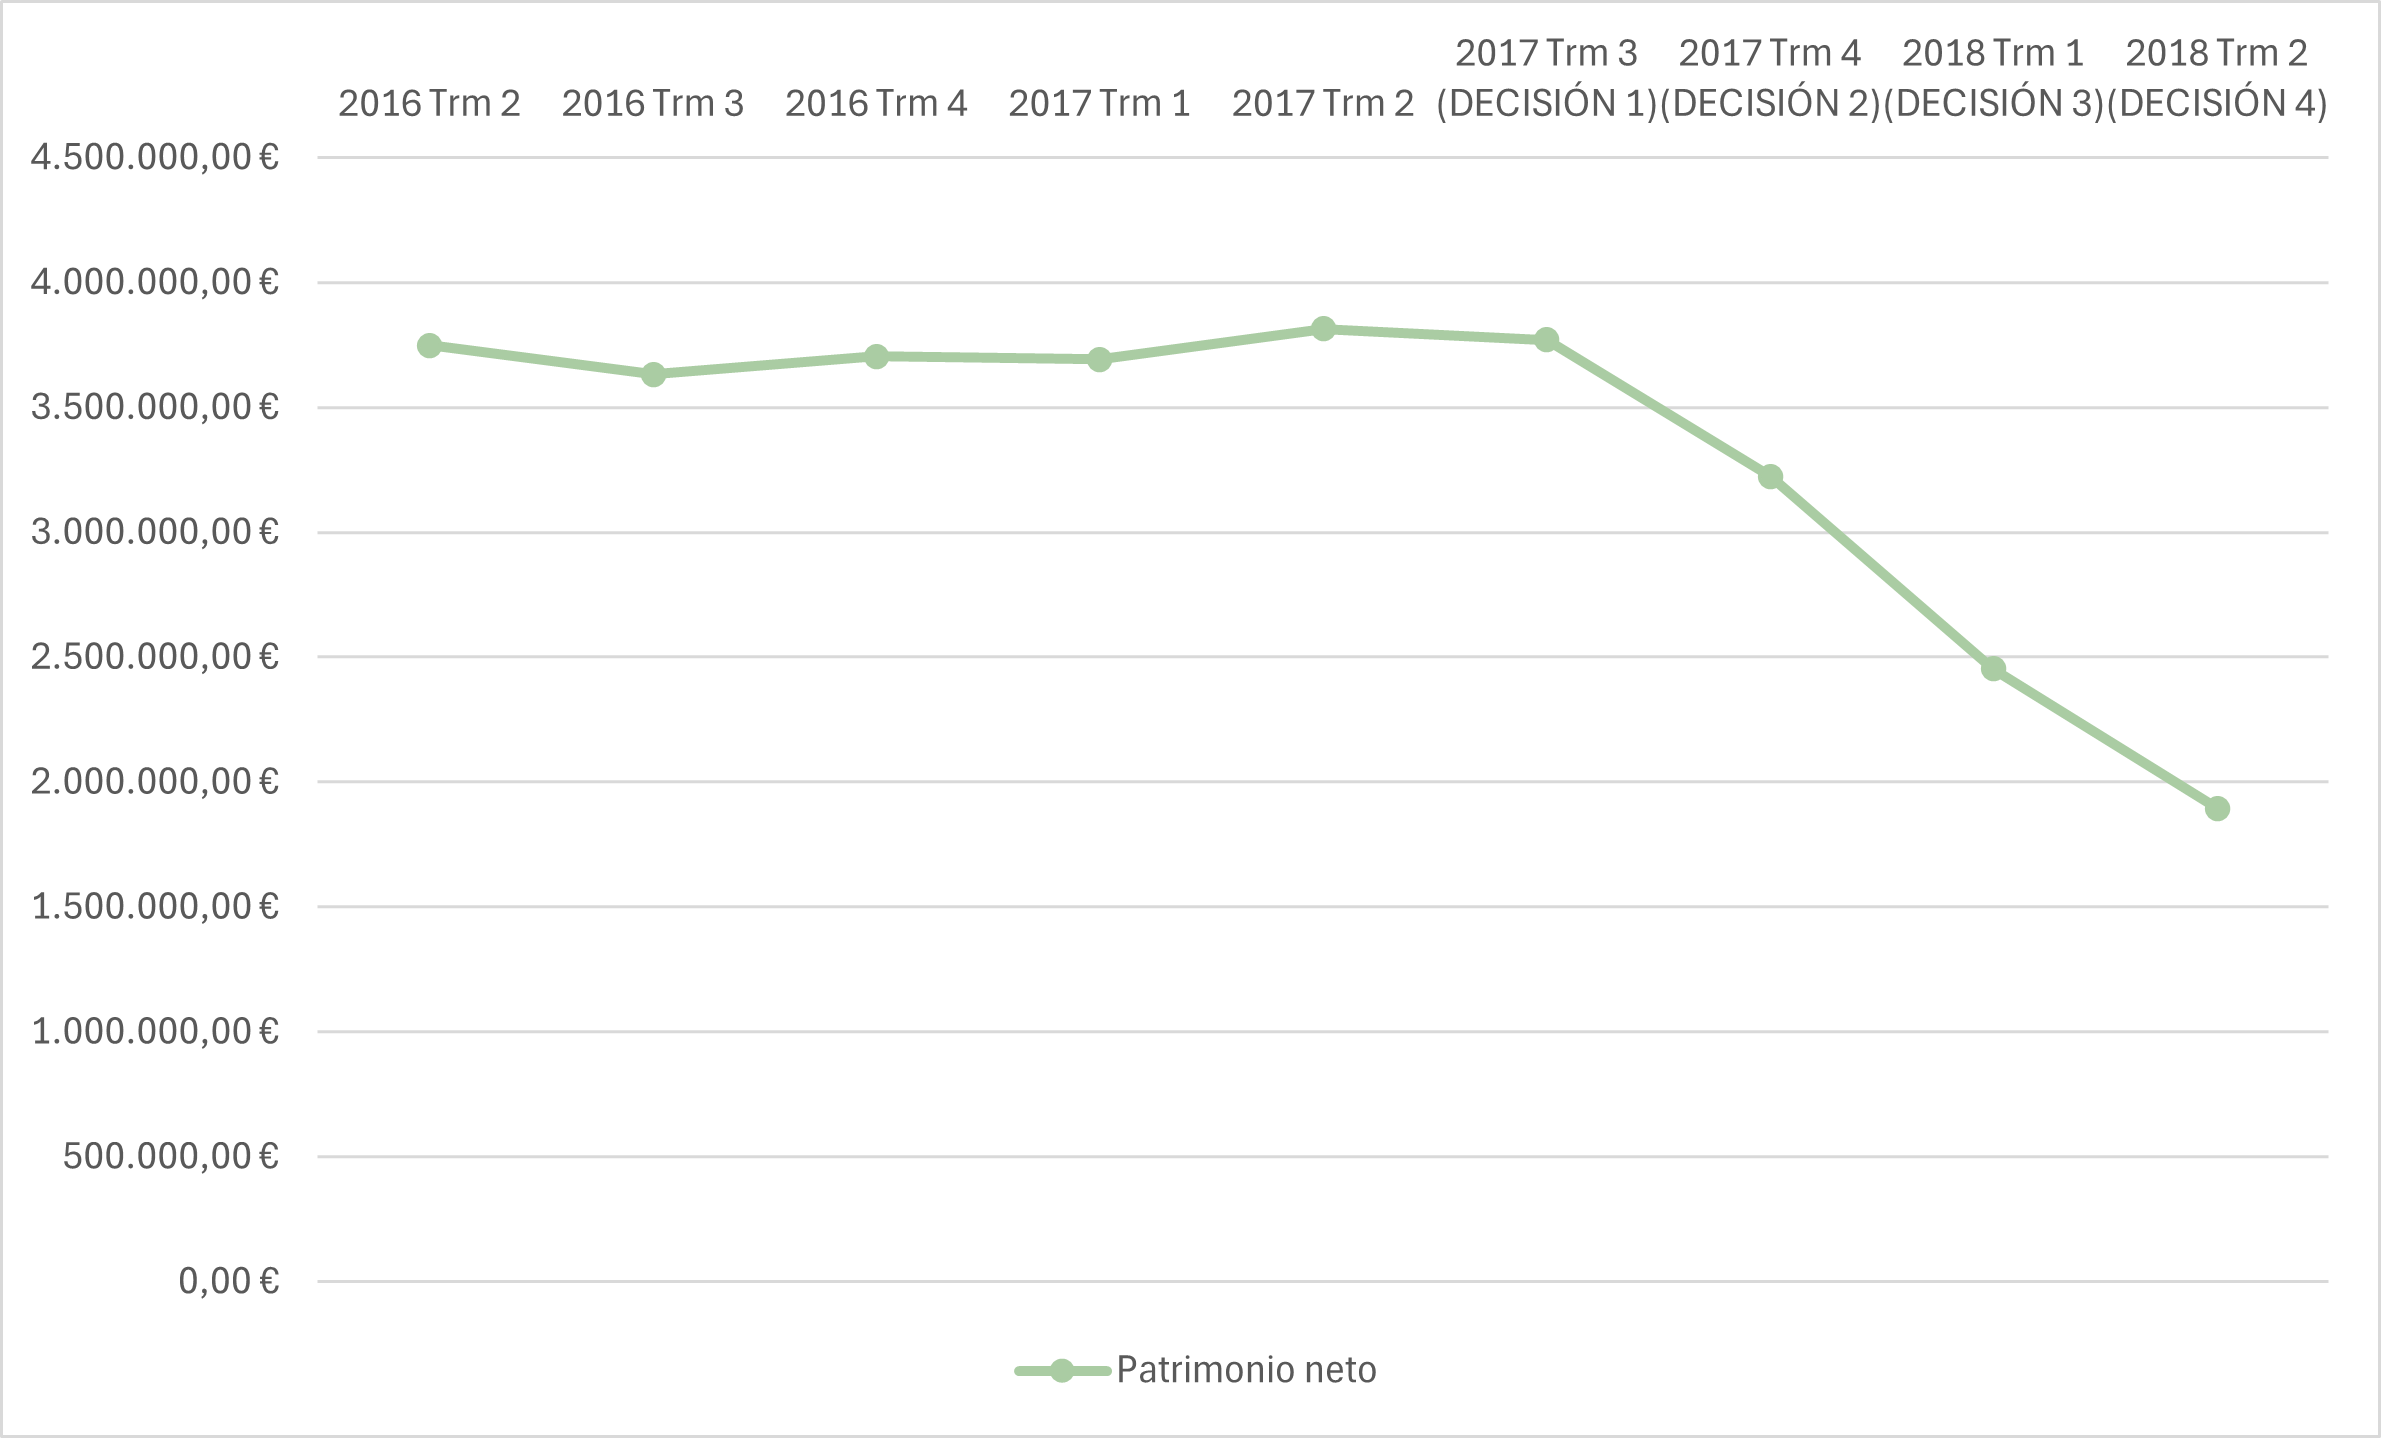
\includegraphics[width= \columnwidth]{Imagenes/decision4_patrimonioneto.png}
\end{figure}

El análisis de solvencia que se puede realizar con el Fondo de Maniobra muestra un desequilibrio severo, teniendo un valor de -1.488.110€. IndusMoney tiene muchas mas deudas a corto plazo, debido al descubierto bancario y los proveedores, que activos corrientes. Esto sitúa a la empresa en una dependencia casi exclusiva de su capacidad para liquidar el stock y transformarlo en liquidez con el que poder reducir el descubierto bancario. Cualquier retraso en la rotación de estos inventarios significará, inevitablemente, el fin de la capacidad operativa de la empresa.

\begin{figure}[h]
  \centering
  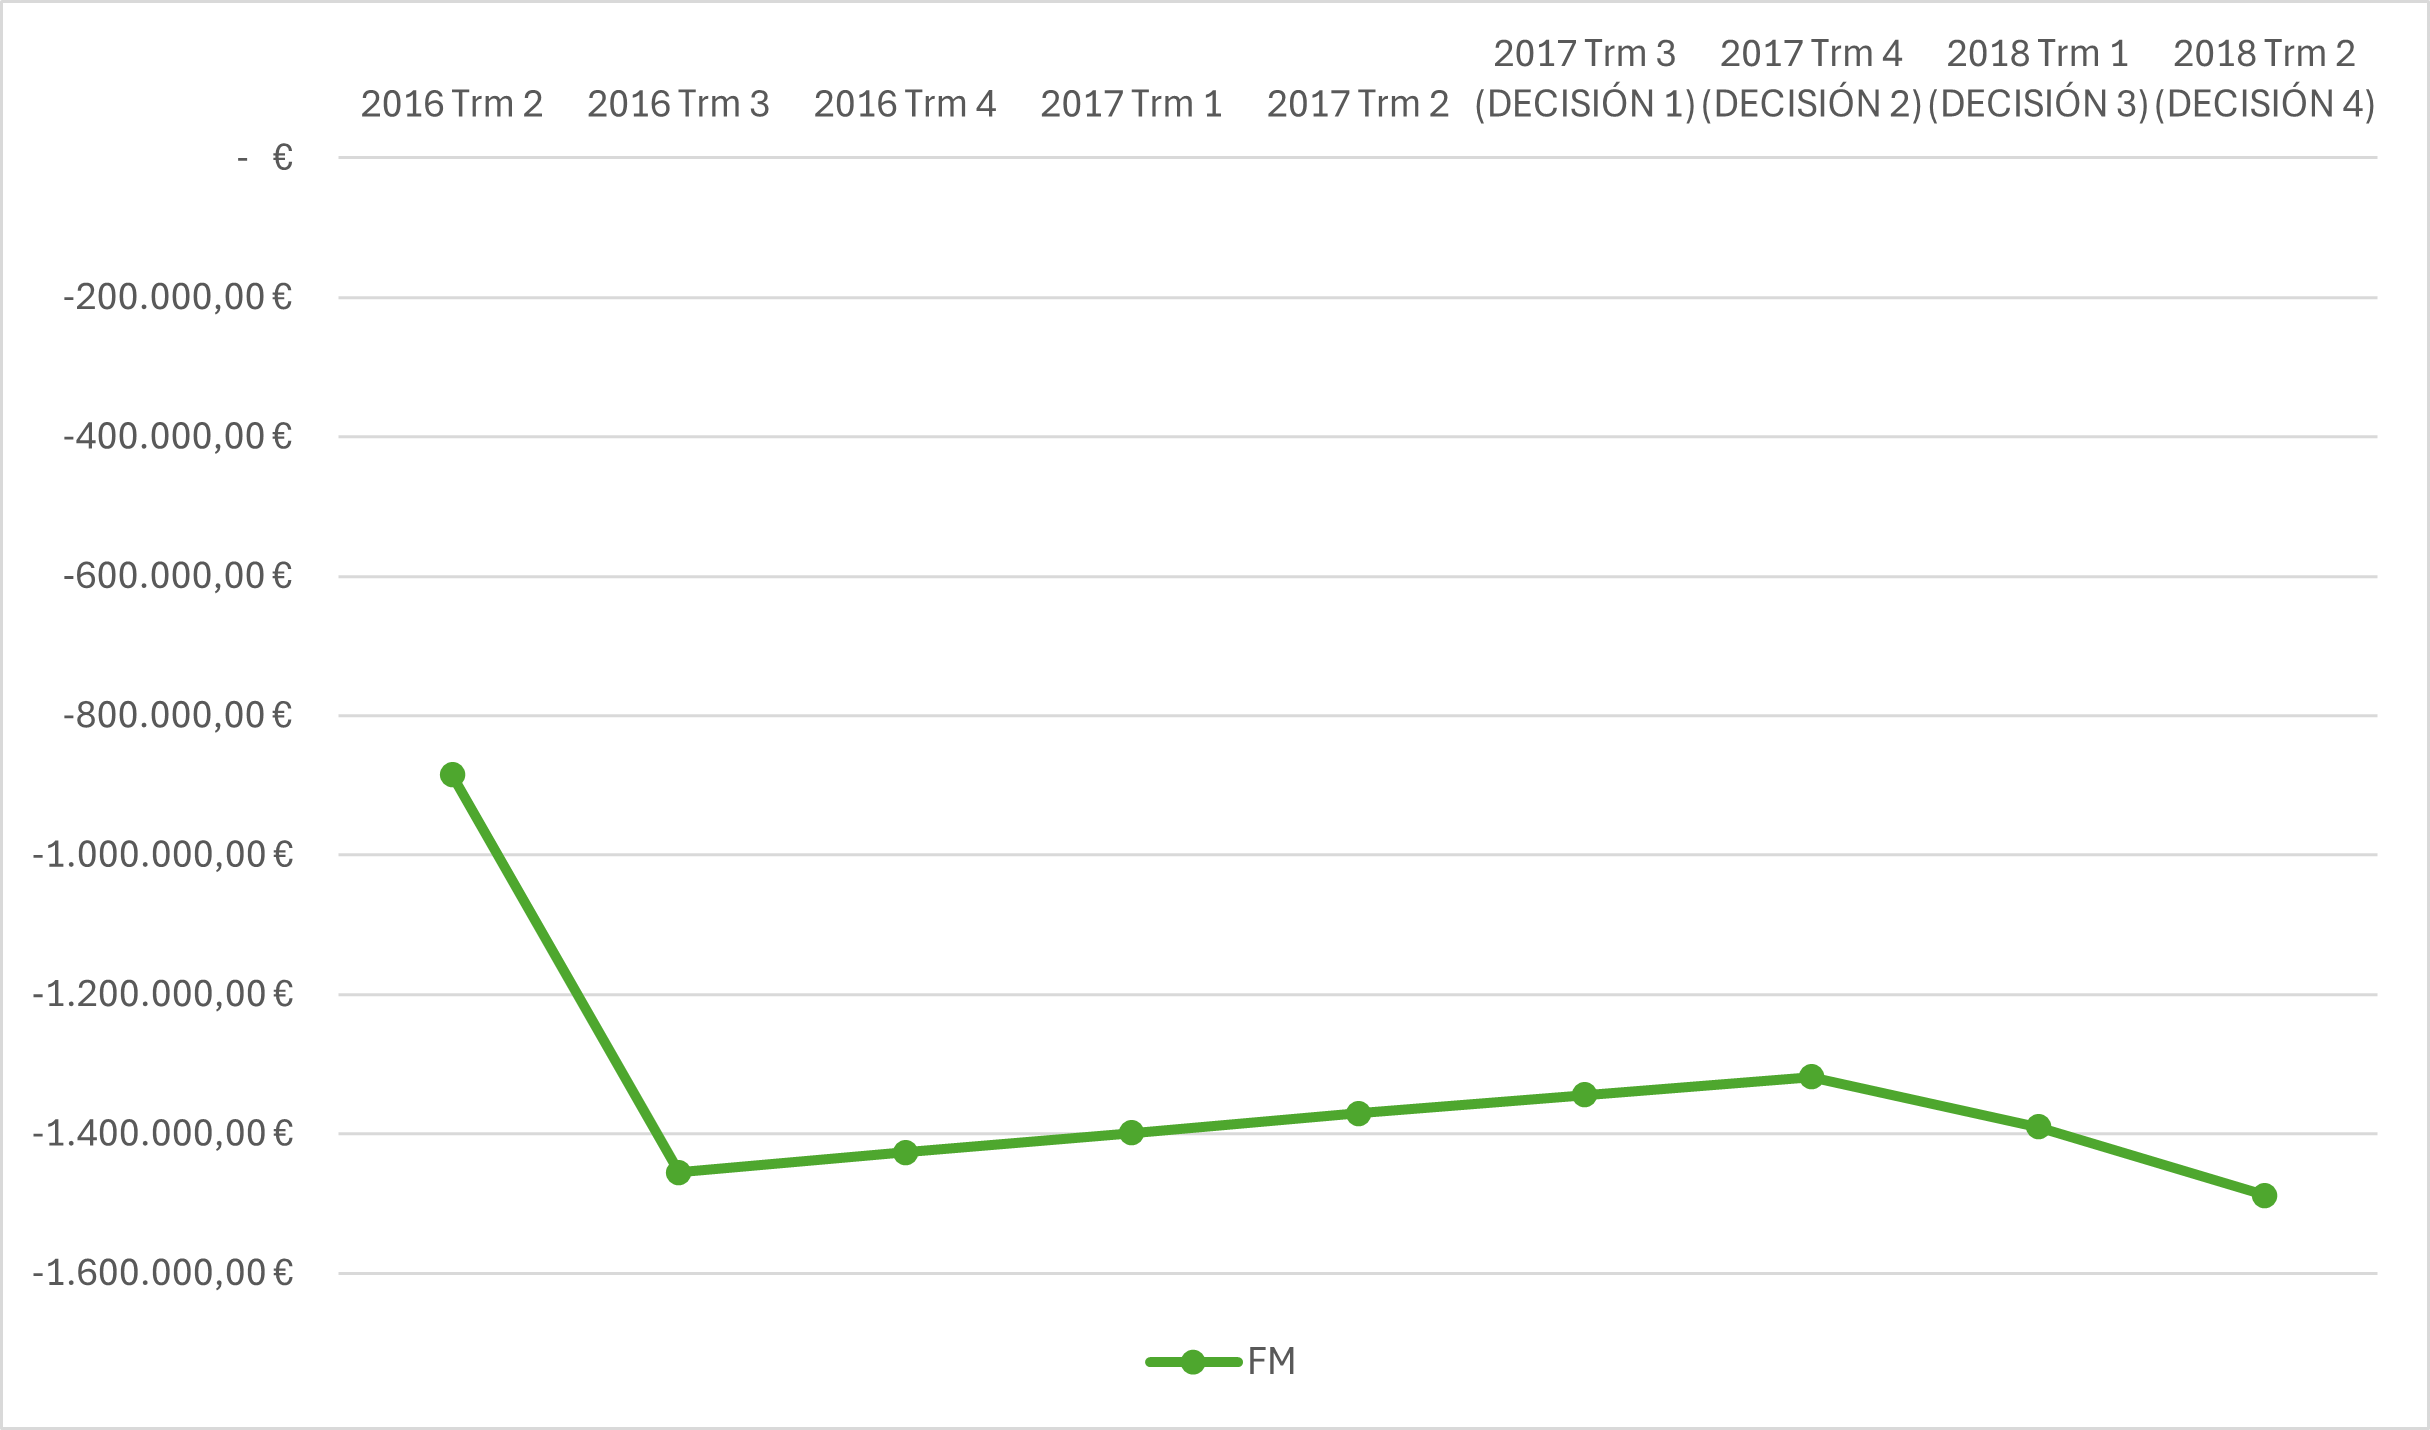
\includegraphics[width= \columnwidth]{Imagenes/decision4_FM.png}
\end{figure}

\section*{Una Estructura Insostenible}
Al cierre del segundo semestre, IndusMoney presenta una situación de exceso de deuda y stock. La estrategia de expansión y sobreabastecimiento ha creado una situación de cuello de botella financiero. La empresa se enfrenta en el siguiente trimestre a almacenes llenos de materia prima, pero con la caja completamente vacía y una deuda bancaria. 

\begin{table}[h]
    \centering
    \begin{tabular}{lr}
        \textbf{Balance - 4ª Decisión}               & \textbf{€} \\
        \hline
        \textbf{Activo fijo}                & \\
        Terreno                             & 50000 \\
        Bienes inmuebles                    & 400000 \\
        Valor de las máquinas               & 1538110 \\
        \cline{2-2}
        \textbf{Total activo fijo}          & \textbf{1988110} \\
        \textbf{Activo Circulante}          & \\
        Inventario - Productos              & 3740 \\
        Inventario - Componentes            & 18990 \\
        Inventario - Materia Prima          & 2275022 \\
        Deudores                            & 375306 \\
        Efectivo e Inversores               & 0 \\
        \cline{2-2}
        \textbf{Total activo circulante}    & \textbf{2673058} \\
        \cline{2-2}
        \textbf{Activo Total}               & \textbf{4661168} \\
        \textbf{Pasivo:}                    & \\
        Impuestos a pagar                   & 0 \\
        Acreedores                          & 864599 \\
        Línea de crédito / Descubierto      & 1401318 \\
        \cline{2-2}
        \textbf{Pasivo exigible}            & \textbf{2265917} \\
        \textbf{Préstamos}                  & \textbf{500000} \\
        \textbf{Activo neto}                & \textbf{1895251} \\
        \textbf{Fondos propios}             & \\
        Capital social                      & 4000000 \\
        Prima de emisión                    & 0 \\
        Reservas                            & -2104749 \\
        \cline{2-2}
        \textbf{Patrimonio neto}            & 1895251 
    \end{tabular}
\end{table}

\begin{table}[h]
    \centering
    \begin{tabular}{|c|r|}
        \hline
        NOF & 407.141,00 € \\
        FM & -1.488.110,00 € \\
        EC & -1.895.251,00 € \\
        \hline
    \end{tabular}
\end{table}